\documentclass[11pt]{article}
\usepackage[margin=1in]{geometry}
\usepackage{amsmath,amssymb,amsthm,mathtools}
\usepackage{booktabs,array,multirow}
\usepackage{graphicx}
\usepackage[numbers,sort&compress]{natbib}
\usepackage{xcolor}
\usepackage[colorlinks=true,linkcolor=blue!50!black,citecolor=blue!50!black,urlcolor=blue!50!black]{hyperref}
\usepackage[capitalise,nameinlink]{cleveref}
\usepackage{enumitem}
\usepackage{algorithm}
\usepackage{algpseudocode}

\newcommand{\SoftwareVersion}{2.0.0@33ad5e4}
\newcommand{\PaperDate}{November 5, 2026}
\newcommand{\EtwoGainMtwoVsMzero}{0.0272}
\newcommand{\EtwoBatterScale}{0.50}
\newcommand{\EtwoPitcherScale}{0.75}
\newcommand{\EtwoHalfLife}{365}
\newcommand{\EtwoBoundaryNote}{all three selected values are interior to the final grid}
\newcommand{\EtwoHalfLifeGrid}{180, 270, 365, 730, 1095}
\newcommand{\EtwoBatterGain}{0.017}
\newcommand{\EtwoPitcherGain}{0.010}
\newcommand{\EtwoTuneGain}{0.0010}
\newcommand{\EtwoMthreeA}{$-$0.0011}
\newcommand{\EtwoMthreeALo}{$-$0.0015}
\newcommand{\EtwoMthreeAHi}{$-$0.0007}
\newcommand{\EtwoMthreeB}{$-$0.0002}
\newcommand{\EtwoMthreeBLo}{$-$0.0006}
\newcommand{\EtwoMthreeBHi}{$+$0.0001}
\newcommand{\EzeroN}{60}
\newcommand{\EzeroMatch}{60}
\newcommand{\EtwocN}{300}
\newcommand{\EtwocSame}{3.0\%}
\newcommand{\EtwocLoss}{0.0073}
\newcommand{\EtwocLossMax}{0.0379}
\newcommand{\EtwocUpTwo}{0.0197}
\newcommand{\EtwocUpThree}{0.0196}
\newcommand{\EtwocCorr}{0.841}
\newcommand{\EthreeSlope}{0.94}
\newcommand{\EthreeSlopeLo}{0.81}
\newcommand{\EthreeSlopeHi}{1.06}
\newcommand{\EthreeBias}{$-$0.035}
\newcommand{\EthreeBiasLo}{$-$0.096}
\newcommand{\EthreeBiasHi}{$+$0.026}
\newcommand{\EthreeN}{9{,}860}
\newcommand{\EthreeCorr}{0.151}
\newcommand{\EthreeMseModel}{9.459}
\newcommand{\EthreeMseConst}{9.680}
\newcommand{\EthreeMseTeam}{9.781}
\newcommand{\EthreeCoverage}{82.7\%}
\newcommand{\EthreeCoverageModel}{85.5\%}
\newcommand{\EthreeShort}{12}
\newcommand{\EthreeCoverageZ}{$-$1.4}
\newcommand{\EthreePitN}{300}
\newcommand{\EfourbN}{9{,}860}
\newcommand{\EfourbUpliftMean}{0.020}
\newcommand{\EfourbUpliftMedian}{0.018}
\newcommand{\EfourbUpliftQninety}{0.033}
\newcommand{\EfourbUpliftMax}{0.080}
\newcommand{\EfourbUpliftSE}{0.0001}
\newcommand{\EfourbUpliftSeason}{3.2}
\newcommand{\EfourbSpread}{0.094}
\newcommand{\EfourbOptVsRandom}{0.050}
\newcommand{\EfourbPctMedian}{97.8\%}
\newcommand{\EfourbPctMean}{94.0\%}
\newcommand{\EfourbShareAboveNinety}{82\%}
\newcommand{\EfourbBookGap}{0.009}
\newcommand{\EfourbRvGap}{0.009}
\newcommand{\EfourbObpGap}{0.011}
\newcommand{\EfouraExhaustiveSeconds}{1.40}
\newcommand{\EfouraN}{200}
\newcommand{\EfouraCurse}{0.164}
\newcommand{\EfouraNoisyGap}{0.0223}
\newcommand{\EfouraActualSameGap}{0.0240}
\newcommand{\EfouraNoisyN}{30}
\newcommand{\EfourcN}{80}
\newcommand{\EfourcDraws}{40}
\newcommand{\EfourcPBetter}{87.3\%}
\newcommand{\EfourcExcl}{33.8\%}
\newcommand{\EfourcSame}{0.5\%}
\newcommand{\EfourcWidth}{0.051}
\newcommand{\RefAwayTeam}{Milwaukee Brewers}
\newcommand{\RefUpliftAway}{$+$0.010}
\newcommand{\RefActualAway}{3.833}
\newcommand{\RefOptimalAway}{3.843}
\newcommand{\RefPctAway}{97.9\%}
\newcommand{\RefBookAway}{3.837}
\newcommand{\RefWorstAway}{3.789}
\newcommand{\RefLoAway}{$-$0.002}
\newcommand{\RefHiAway}{$+$0.021}
\newcommand{\RefPBetterAway}{91.2\%}
\newcommand{\RefSameAway}{0.2\%}
\newcommand{\RefRegretAway}{0.013}
\newcommand{\RefCertAway}{8.2\times10^{-5}}
\newcommand{\RefObservedAway}{4}
\newcommand{\RefHomeTeam}{Tampa Bay Rays}
\newcommand{\RefUpliftHome}{$+$0.024}
\newcommand{\RefActualHome}{3.336}
\newcommand{\RefOptimalHome}{3.360}
\newcommand{\RefPctHome}{99.3\%}
\newcommand{\RefBookHome}{3.347}
\newcommand{\RefWorstHome}{3.246}
\newcommand{\RefLoHome}{$+$0.009}
\newcommand{\RefHiHome}{$+$0.041}
\newcommand{\RefPBetterHome}{99.5\%}
\newcommand{\RefSameHome}{9.5\%}
\newcommand{\RefRegretHome}{0.005}
\newcommand{\RefCertHome}{5.4\times10^{-4}}
\newcommand{\RefObservedHome}{1}
\newcommand{\RefDraws}{400}
\newcommand{\RefQmin}{0.633}
\newcommand{\RefTruncBound}{1.7\times10^{-11}}
\newcommand{\DataErrMin}{0}
\newcommand{\DataErrMax}{1}
\newcommand{\EoneStateZeroMaxDiff}{0.007}
\newcommand{\EoneWeightedDiff}{0.011}
\newcommand{\EoneMaxDiff}{0.20}
\newcommand{\EoneREzero}{0.491}
\newcommand{\EoneFiveSingle}{18.7\%}
\newcommand{\EoneFiveK}{19.9\%}
\newcommand{\EoneAllSingle}{14.1\%}
\newcommand{\EoneAllK}{22.6\%}
\newcommand{\EoneFiveImmDiff}{0.014}


\newtheorem{theorem}{Theorem}
\newtheorem{proposition}[theorem]{Proposition}
\newtheorem{lemma}[theorem]{Lemma}
\newtheorem{corollary}[theorem]{Corollary}
\theoremstyle{definition}
\newtheorem{definition}{Definition}
\newtheorem{assumption}{Assumption}
\renewcommand{\theassumption}{A\arabic{assumption}}
\crefname{assumption}{Assumption}{Assumptions}
\Crefname{assumption}{Assumption}{Assumptions}
\crefname{proposition}{Proposition}{Propositions}
\crefname{lemma}{Lemma}{Lemmas}
\crefname{corollary}{Corollary}{Corollaries}
\crefname{theorem}{Theorem}{Theorems}
\crefname{remark}{Remark}{Remarks}
\crefname{definition}{Definition}{Definitions}
\theoremstyle{remark}
\newtheorem{remark}{Remark}

\newcommand{\E}{\mathbb{E}}
\renewcommand{\P}{\mathbb{P}}
\newcommand{\R}{\mathbb{R}}
\newcommand{\cS}{\mathcal{S}}
\newcommand{\cC}{\mathcal{C}}
\newcommand{\cF}{\mathcal{F}}
\newcommand{\cI}{\mathcal{I}}
\newcommand{\one}{\mathbf{1}}
\newcommand{\abs}{\mathsf{a}}
\DeclareMathOperator*{\argmax}{arg\,max}

\title{How Much Does the Batting Order Matter?\\[2pt]
\large Exact Expected-Runs Optimization with an Empirical-Bayes Plate-Appearance Model,\\
and the 2026 World Series}
\author{Fernando Gonz\'alez\thanks{Code, data-processing scripts and the interactive dashboard:
\url{https://github.com/fernandogg2004/mlb-lineup-optimizer}. Software version \texttt{\SoftwareVersion}.}}
\date{\PaperDate}

\begin{document}
\maketitle

\begin{abstract}
We study the choice of a batting order for a fixed set of nine hitters, with the objective of
maximizing the expected number of runs scored in nine offensive innings. Each hitter's
plate-appearance outcome distribution against the opposing starting pitcher and bullpen is
estimated, using only information available before the game, by an empirical-Bayes
multiplicative (log5-type) model fitted to Statcast data. Base-out transitions, including
base-running between plate appearances, are estimated from the data rather than assumed. Under
explicit Markov assumptions the expected runs of a lineup can be computed exactly through an
inning-level Markov chain on the leadoff slot; we prove that the computation is well defined,
bound its truncation error, and use rotational structure to evaluate all $9!=362{,}880$ orders in
about \EfouraExhaustiveSeconds{} seconds, so that the reported optimum is certified within the model.
On held-out seasons (2025--2026) the plate-appearance model improves log-loss over the league
baseline by \EtwoGainMtwoVsMzero{} nats per plate appearance, and the run predictions are
calibrated (slope \EthreeSlope{}). Over \EfourbN{} team-games, the model-optimal order exceeds the
order actually used by \EfourbUpliftMean{} expected runs per game (\EfourbUpliftSeason{} per
162 games), and actual orders rank, on median, above \EfourbPctMedian{} of all possible orders.
For Game~5 of the 2026 World Series (Milwaukee~4, Tampa Bay~1) the estimated gains are
\RefUpliftAway{} (Milwaukee) and \RefUpliftHome{} (Tampa Bay) runs per game, with 90\% parameter-
uncertainty intervals that are of the same order as the gains themselves. These are model-based
counterfactuals: a historical game reveals only the outcome of the order that was used, so no
observed result can confirm them.
\end{abstract}

\tableofcontents

%======================================================================
\section{Introduction}
%======================================================================

Batting-order construction is among the oldest quantitative questions in baseball and a classical
application of Markov chains and simulation in operations research
\cite{lindsey1963,freeze1974,cover1977,dEsopo1977,pankin1978,bukiet1997,sokol2003}. The
received wisdom from that literature, popularized by \citet{tango2007}, is that the order matters,
but only modestly: a sensible order is worth only a few runs per season less than the best one.

This paper re-derives that conclusion with three ingredients that we found missing from the
software system it replaces:
\begin{enumerate}[leftmargin=*]
\item \textbf{A precisely defined objective.} We maximize $\E[R_9\mid\pi,\cI]$, the expected runs
in nine offensive innings for a fixed pregame order $\pi$ given the information $\cI$ available
before first pitch. We do \emph{not} optimize win probability, which at the level of a single game
is close to a coin flip and depends on the opponent's offense as well.
\item \textbf{Exact evaluation and exhaustive search.} The predecessor system ranked orders by
Monte Carlo estimates inside a genetic algorithm. Because selection among noisy estimates is
biased upward (the ``optimizer's curse'' \cite{smith2006}), it could not certify that its output
was optimal, and it overstated the gain of the selected order. We evaluate expected runs exactly
(\cref{sec:model}) and search all orders exhaustively (\cref{sec:optimization}).
\item \textbf{Leakage-free, falsifiable validation.} All estimates for a game on date $d$ use only
plate appearances before $d$. We validate the plate-appearance model on held-out seasons, check
that the implied run expectancy matches observed scoring, and check the calibration of game-level
run predictions (\cref{sec:experiments,sec:results}).
\end{enumerate}

\paragraph{What the paper does not claim.} The value of an unplayed order cannot be observed:
a historical game shows the runs scored under the order the manager chose, not under any other.
Every comparison between orders in this paper is therefore a statement \emph{about the model}.
We validate the model's ingredients on observed data and quantify parameter uncertainty, but we
make no causal claim that a team would have scored more runs (\cref{rem:identification}).

\paragraph{Contribution.} The mathematical tools are classical: absorbing Markov chains
\cite{kemeny1960}, the base-out run-expectancy framework \cite{lindsey1963,tango2007}, and
empirical-Bayes shrinkage \cite{efron1975,brown2008}. Our contribution is an end-to-end,
reproducible implementation that (i) estimates the transition kernel and batter-specific outcome
distributions without future information, (ii) evaluates lineups exactly with a proven error
bound, (iii) certifies the optimum by exhaustive search, and (iv) reports uncertainty and
validation honestly, including null and small effects. We do not claim mathematical novelty for
the individual propositions; several are elementary consequences of standard theory, and we say
so where relevant.

%======================================================================
\section{Problem formulation}\label{sec:formulation}
%======================================================================

\subsection{Players, orders and feasibility}

A lineup consists of nine hitters indexed by $i\in\{1,\dots,9\}$. A batting order is a bijection
$\pi:\{1,\dots,9\}\to\{1,\dots,9\}$ assigning hitter $\pi(t)$ to slot $t$; the set of all orders is
the symmetric group $\mathcal{S}_9$, with $|\mathcal{S}_9|=362{,}880$. Under the Official Baseball
Rules any order of the nine starters is legal, and with the universal designated hitter (adopted by
MLB in 2022) the pitcher does not bat, so the feasible set is $\cF=\mathcal{S}_9$. Users of the
dashboard may add constraints of the form ``hitter $i$ bats in slot $t$''; these define
$\cF_A=\{\pi:\pi(t)\in A_t\ \forall t\}$ for allowed sets $A_t$.

We consider a \emph{fixed pregame} order. In-game substitutions, pinch hitting and defensive
changes are outside the model: the nine starters bat throughout.

\subsection{State space and outcomes}

\begin{definition}[Base-out states]
A transient state is a pair $s=(o,b)$ with $o\in\{0,1,2\}$ outs and $b\in\{0,1\}^3$ the occupancy
of first, second and third base. We encode $s=8o+b_1+2b_2+4b_3\in\{0,\dots,23\}$ and add an absorbing
state $\abs$ (three outs). Let $\cS=\{0,\dots,23\}$ and $\bar\cS=\cS\cup\{\abs\}$.
\end{definition}

\begin{definition}[Outcome classes]
The batter-specific result of a plate appearance (PA) is one of eight classes
$\cC=\{\mathrm{K},\mathrm{BB},\mathrm{1B},\mathrm{2B},\mathrm{3B},\mathrm{HR},\mathrm{GB},\mathrm{AIR}\}$:
strikeout; walk, intentional walk, hit-by-pitch or catcher's interference; single; double; triple;
home run; a ground ball not scored as a hit (including double plays, fielder's choices and
reaching on an error); and a fly ball, line drive or pop-up not scored as a hit (including
sacrifice flies).
\end{definition}

Splitting non-hit balls in play by batted-ball type lets the model distinguish hitters who ground
into double plays from those who hit sacrifice flies, without modelling either event per hitter.

\begin{definition}[Transition kernel]\label{def:kernel}
For $c\in\cC$, $s\in\cS$, $s'\in\bar\cS$ and $r\in\{0,\dots,4\}$, $J_c(s,s',r)$ is the probability
that, from state $s$, a PA with outcome $c$ (together with all base-running events up to the
decisive pitch of the next PA) leads to $s'$ with $r$ runs scored. We write
$P_c(s,s')=\sum_r J_c(s,s',r)$ and $\rho_c(s)=\sum_{s',r}r\,J_c(s,s',r)$.
\end{definition}

Defining a transition from one decisive pitch to the next (\cref{sec:data}) means stolen bases,
pick-offs and wild pitches are part of the kernel, and an inning that ends on a caught stealing
correctly leaves the batter at the plate to lead off the next inning.

\subsection{Stochastic model}

Fix an order $\pi$. Pitching regimes $g\in\{1,\dots,G\}$ index who pitches (here $G=2$: the
opposing starter and the opposing bullpen). Let $x_g(i)\in\Delta(\cC)$ be the outcome distribution
of hitter $i$ under regime $g$, and $w_k\in\Delta(\{1,\dots,G\})$ the regime distribution of inning
$k\in\{1,\dots,9\}$.

\begin{assumption}[Markov plate appearances]\label{as:markov}
Within a half-inning pitched under regime $g$, given the current state $S_n=s$ and the batting
slot $T_n=t$, the outcome $C_n\sim x_g(\pi(t))$ and the next state and runs
$(S_{n+1},\,\Delta R_n)\sim J_{C_n}(s,\cdot,\cdot)$ are independent of everything else that
happened before; then $T_{n+1}=T_n+1 \pmod 9$.
\end{assumption}

\begin{assumption}[Batter-independent kernel]\label{as:kernel}
$J_c$ does not depend on the identity of the batter or runners; base running is league-average.
\end{assumption}

\begin{assumption}[Pitching changes between innings]\label{as:regime}
The regime $G_k$ of inning $k$ is drawn from $w_k$ independently of the game state and of
other innings, and does not change within an inning.
\end{assumption}

\begin{assumption}[Outs]\label{as:outs}
Outs never decrease within an inning, and there is $q>0$ such that every PA increases the number
of outs with probability at least $q$ whatever the state, hitter and regime:
$\min_{g,i,s}\sum_{c}x_g(i)_c\sum_{s':\,o(s')>o(s)}P_c(s,s')\ge q$, with $o(\abs)=3$.
\end{assumption}

\begin{assumption}[Bookkeeping]\label{as:bookkeeping}
Every transition conserves participants: if $s'\ne\abs$, $|b(s)|+1=|b(s')|+r+o(s')-o(s)$; if
$s'=\abs$, $r+3-o(s)\le|b(s)|+1$.
\end{assumption}

\Cref{as:outs,as:bookkeeping} are checked on the estimated kernel: no observed transition decreases
the outs, and every transition violating the identity is a data error and is removed
(\cref{sec:data}). Each inning starts in state $s=0$ (no outs, bases empty); the extra-inning
runner rule is irrelevant for a nine-inning objective.

Let $R_9=\sum_{k=1}^9 R^{(k)}$ be the runs scored in the first nine innings, where $R^{(k)}$ is the
total of $\Delta R_n$ in inning $k$.

\begin{definition}[Objective]
For an information set $\cI$ (all data before the game date), the expected-runs objective is
\[
V(\pi)=\E\bigl[R_9\mid \pi,\cI\bigr],\qquad \pi^\star\in\argmax_{\pi\in\cF}V(\pi),
\]
where the expectation is with respect to the model of \cref{as:markov,as:kernel,as:regime} with
parameters $\theta=(J,x,w)$ replaced by their estimates $\hat\theta$ from $\cI$
(\cref{sec:estimation}); $V=V_{\hat\theta}$ is a plug-in value, not a posterior-predictive
expectation. Independence of the regimes across innings (\cref{as:regime}) is a simplification
(a starter who has left does not return), and $w_k$ is interpretable as the probability that the
starter pitches inning $k$ only under it. Expected runs per inning
($V/9$) and per plate appearance are derived quantities; win probability is not modelled.
\end{definition}

\begin{remark}[Identification]\label{rem:identification}
For a historical game we observe one realization of $R$ under the order $\pi_{\mathrm{used}}$.
$V(\pi)$ for $\pi\ne\pi_{\mathrm{used}}$ is a counterfactual expectation that is identified only
through the structural assumptions above. Assumptions A1--A3 are what make the order affect runs
only through the sequence in which hitters come to the plate; they cannot be tested on games
played under a single order. Moreover, the predicted gain of reordering (hundredths of a run) is
two orders of magnitude smaller than the standard deviation of a team's runs in one game
(about 3), so no feasible observational study could detect it reliably.
\end{remark}

%======================================================================
\section{Statistical estimation}\label{sec:estimation}
%======================================================================

\subsection{Data}\label{sec:data}

We use pitch-level Statcast data (Baseball Savant \cite{savant}) for 2021--2026, regular season and postseason,
downloaded in two-day windows and stored unmodified, with SHA-256 manifests. For each PA the
decisive pitch is the pitch with a non-empty \texttt{events} field; its fields
\texttt{outs\_when\_up}, \texttt{on\_1b/2b/3b} and \texttt{bat\_score} give the state and score
before the decisive pitch. The transition of PA $n$ is from its decisive state to the decisive
state of PA $n+1$ in the same half-inning, or to $\abs$ for the last PA; its runs are the change in
the batting team's score (for the last PA, up to the score at the end of the half-inning).
Plate appearances interrupted by the end of an inning (\texttt{truncated\_pa}) are not PAs. The
final transition of a game's last half-inning is censored, and excluded from estimation, unless
the game ended normally after three outs (a top half of the ninth or later with the home team ahead,
or a bottom half with the visitors ahead); this covers walk-offs in any inning, called games and
seven-inning games. Censoring is outcome-dependent (walk-off transitions score runs by
construction), but it affects about one transition in a thousand.

Starting lineups are inferred as the first nine distinct batters of each team; the inference is
marked reliable when the tenth PA returns to the leadoff hitter. In a random audit of \EzeroN{}
reliable 2026 team-games (E0) the inferred lineup and opposing starter matched the official boxscore
in \EzeroMatch{} of them. For the
reference game we use the official boxscore (slot codes $100,\dots,900$).
\Cref{tab:data} summarizes the data.

\begin{table}[t]\centering\small
\caption{Statcast data after processing (regular season and postseason). Non-conserving: bookkeeping violations outside censored transitions (data errors).}\label{tab:data}
\begin{tabular}{lrrrrr}\toprule
Season & Games & PAs & Reliable lineups & Censored & Non-conserving\\\midrule
2021 & 2,466 & 184,592 & 4,919/4,932 & 339 & 0 \\
2022 & 2,470 & 185,047 & 4,923/4,940 & 222 & 1 \\
2023 & 2,471 & 187,190 & 4,924/4,942 & 196 & 0 \\
2024 & 2,472 & 185,715 & 4,928/4,944 & 215 & 0 \\
2025 & 2,477 & 186,562 & 4,948/4,954 & 230 & 0 \\
2026 & 2,469 & 186,777 & 4,924/4,938 & 205 & 1 \\
\bottomrule\end{tabular}\end{table}


\subsection{Transition kernel}

For a game on date $d$, let $m(d)$ be the first day of its month. The kernel is refitted monthly:
$N_c(s,s',r)$ counts valid transitions in the window
$[\max(m(d)-1095\text{ days},\ \text{2023-01-01}),\,m(d))$ (if that window would span less than
180 days, the previous 365 days are used instead). Refitting monthly only discards information and
cannot introduce look-ahead. The 2023 lower limit reflects the 2023 rule
changes (larger bases, pick-off limits, defensive-shift restrictions), which changed base-running
and batted-ball outcomes. The estimate is the Dirichlet posterior mean
\[
\hat J_c(s,\cdot,\cdot)=\frac{N_c(s,\cdot,\cdot)+\alpha J^0_c(s,\cdot,\cdot)}{N_c(s)+\alpha},
\qquad \alpha=2,
\]
centred on the conventional deterministic advancement $J^0$ (runners advance one base on a
single, a ground ball with a runner on first and fewer than two outs is a double play, other outs
do not advance runners). The prior only matters in sparse cells.

\subsection{Plate-appearance model}

Let $h=(\text{batter side},\text{pitcher hand})$ denote the handedness matchup and
$\ell_h\in\Delta(\cC)$ the league outcome distribution for $h$. For hitter $b$ facing pitcher $p$
we model
\begin{equation}\label{eq:log5}
\varphi(c\mid b,p)=\frac{\ell_h(c)\,m_b(c)\,m_p(c)}{\sum_{c'}\ell_h(c')\,m_b(c')\,m_p(c')},
\end{equation}
a multinomial generalization of the odds-ratio (``log5'') method introduced by
\citet{james1981} and discussed by \citet{tango2007}, with batter
and pitcher multipliers $m_b,m_p\in(0,\infty)^{\cC}$. Platoon effects enter only through the
league distribution $\ell_h$; individual platoon splits are not estimated, because they stabilize
only after very large samples \cite{tango2007}.

\paragraph{Empirical-Bayes multipliers.} Each PA in the 1{,}095 days before the cutoff receives a weight
$\omega=2^{-\text{age}/H}$, where the age is in days and $H$ is a half-life. For hitter $b$ let
$n_b(c)=\sum\omega\,\one\{C=c\}$ and $e_b(c)=\sum\omega\,\ell_{h(\mathrm{PA})}(c)$ over his PAs (the
expected count under league rates). Treating $n_b(c)$ as Poisson with mean $m_b(c)e_b(c)$ and
placing a $\mathrm{Gamma}(a_c,a_c)$ prior (mean one) on $m_b(c)$ gives the posterior
\begin{equation}\label{eq:posterior}
m_b(c)\mid\text{data}\sim\mathrm{Gamma}\bigl(n_b(c)+a_c,\ e_b(c)+a_c\bigr),\qquad
\hat m_b(c)=\frac{n_b(c)+a_c}{e_b(c)+a_c}.
\end{equation}
Multipliers of hitters with little history therefore shrink to one, in the spirit of
\citet{efron1975} and \citet{brown2008}. Pitchers are treated identically with strengths $s_c$.
A team's bullpen is one pseudo-pitcher built from all PAs of pitchers other than that game's
starter. The prior strengths are $a_c=\lambda_B\,\kappa_c$ and $s_c=\lambda_P\,\kappa_c$, with fixed
relative strengths $\kappa=(12,15,40,25,6,12,60,60)$ ordered by how fast each rate stabilizes.
The scales $(\lambda_B,\lambda_P)$ and $H$ are tuned on 2024 only (\cref{sec:experiments}).

\begin{remark}
With fractional weights, the Poisson model in \eqref{eq:posterior} is a working likelihood, not
a literal sampling model: decayed counts are not counts. We use \eqref{eq:posterior} as a shrinkage
rule whose prior strength is tuned out of sample, and the Gamma posterior as an approximate
description of parameter uncertainty (\cref{sec:sensitivity}).
\end{remark}

\paragraph{Starter workload.} For each starting pitcher, $w_k(\text{starter})$ is the decayed average,
over his previous starts, of the share of inning-$k$ plate appearances he faced, shrunk toward the
league curve with a prior of 8 starts. The bullpen pitches the rest. The bullpen distribution for
hitter $b$ mixes \eqref{eq:log5} over pitcher hands in proportion to the bullpen's historical share
of right-handed PAs.

\subsection{Leakage control}

Every quantity above, for a game on date $d$, uses only PAs with $\texttt{game\_date}<d$
(same-day earlier games are excluded). This is enforced in code and tested: altering every PA on
or after $d$ leaves the fitted model bit-for-bit unchanged. Statcast columns that encode the future
(e.g.\ \texttt{pitcher\_days\_until\_next\_game}) are never used.

%======================================================================
\section{Exact evaluation of a batting order}\label{sec:model}
%======================================================================

\subsection{Half-innings as absorbing chains}

Fix a regime $g$ and order $\pi$. Within a half-inning the pair $(S_n,T_n)$ is a Markov chain on
$\bar\cS\times\{1,\dots,9\}$ by \cref{as:markov}. Define the one-PA operator of hitter $i$,
\[
M_g(i)=\sum_{c\in\cC}x_g(i)_c\,P_c\in\R^{24\times 25},\qquad \rho_g(i)=\sum_c x_g(i)_c\,\rho_c\in\R^{24}.
\]

\begin{proposition}[Finite innings]\label{prop:finite}
Under \cref{as:markov,as:outs}, the number $N$ of PAs in a half-inning satisfies
$\P(N>n)\le\P(\mathrm{Bin}(n,q)\le 2)$ for every $n$. In particular $N<\infty$ almost surely,
$\E[N]\le 3/q$, and all moments of $N$ are finite.
\end{proposition}

\begin{proof}
Index PAs from $0$ and let $U_n=\one\{o(S_{n+1})>o(S_n)\}$ for the PA with index $n$. By
\cref{as:outs}, $\P(U_n=1\mid\mathcal{F}_n)\ge q$ on $\{N>n\}$, where $\mathcal{F}_n$ is the history
before PA $n$. Outs never decrease and the inning ends once they reach three, so
$N\le\min\{n:U_0+\dots+U_{n-1}\ge3\}$. A standard coupling (draw
$V_n\sim\mathrm{Unif}(0,1)$ independently and realize $U_n=\one\{V_n<p_n\}$ with
$p_n=\P(U_n=1\mid\mathcal{F}_n)\ge q$; set $B_n=\one\{V_n<q\}\le U_n$) shows that $N$ is
stochastically dominated by the time $T_3$ of the third success in i.i.d.\ Bernoulli$(q)$ trials
$B_n$. Hence $\P(N>n)\le\P(T_3>n)=\P(\mathrm{Bin}(n,q)\le2)$ and $\E[N]\le\E[T_3]=3/q$. Finite
moments follow from the geometric tail of $T_3$.
\end{proof}

\begin{lemma}[Runs are bounded by plate appearances]\label{lem:runs}
Under \cref{as:bookkeeping}, every half-inning satisfies $R^{(k)}+\mathrm{LOB}+3=N$, where LOB is
the number of runners left on base. Hence $R^{(k)}\le N-3$ and $\E[R^{(k)}]\le 3/q-3$.
\end{lemma}

\begin{proof}
Summing the identity of \cref{as:bookkeeping} over the non-absorbing transitions of the inning and
adding the inequality of the absorbing one gives $R^{(k)}+3\le N$. Defining
$\mathrm{LOB}:=|b(S_{N-1})|+1-r_N-(3-o(S_{N-1}))\ge0$ (the participants of the last transition
that neither scored nor were put out) turns this into the identity $R^{(k)}+\mathrm{LOB}+3=N$.
The bound on the expectation follows from \cref{prop:finite}.
\end{proof}

\begin{proposition}[Inning tables]\label{prop:tables}
For a leadoff slot $j$ and regime $g$, let $r_g(j)=\E[R^{(k)}\mid T_1=j,G_k=g]$ and
$L_g(j,j')=\P(\text{slot }j'\text{ leads off the next inning}\mid T_1=j,G_k=g)$. Then, with
$v_0=\mathbf{1}_{\{0\}}^\top$ (all mass on state 0) and $v_{n+1}=v_n M_g(\pi(j+n))_{\cdot,\cS}$,
where slot indices are taken in $\{1,\dots,9\}$ cyclically, $t\mapsto1+((t-1)\bmod 9)$,
\[
r_g(j)=\sum_{n\ge0}v_n\,\rho_g(\pi(j+n)),\qquad
L_g(j,j')=\sum_{n\ge0:\ j+n+1\equiv j'}v_n M_g(\pi(j+n))_{\cdot,\abs},
\]
both series converging geometrically, and $L_g(j,\cdot)$ is a probability vector.
\end{proposition}

\begin{proof}
$v_n(s)$ is the probability that the inning is still in progress at PA $n$ in state $s$ (the slot is
deterministic given $n$). The expected runs of PA $n$ are $v_n\rho_g(\pi(j+n))$, and the inning
ends at PA $n$ with probability $v_nM_g(\cdot)_{\cdot,\abs}$, in which case the next slot,
$j+n+1$, leads off the next inning. Summability and $\sum_{j'}L_g(j,j')=\P(N<\infty)=1$ follow from
\cref{prop:finite}; interchanging sum and expectation is justified by monotone convergence since
runs are non-negative and $\E[R^{(k)}]<\infty$ (\cref{lem:runs}).
\end{proof}

\begin{theorem}[Exact game value]\label{thm:value}
Under \cref{as:markov,as:kernel,as:regime,as:outs,as:bookkeeping}, let
$r_k=\sum_g w_{k,g}r_g$ and $L_k=\sum_g w_{k,g}L_g$. The leadoff slots $(J_k)_{k\ge1}$ of successive
innings form a (time-inhomogeneous) Markov chain with $J_1=1$ and transition matrices $L_k$, and
\begin{equation}\label{eq:value}
V(\pi)=\sum_{k=1}^{9}\mu_k^\top r_k,\qquad \mu_1=e_1,\quad \mu_{k+1}^\top=\mu_k^\top L_k .
\end{equation}
\end{theorem}

\begin{proof}
Every inning starts in state 0, so the only information an inning passes to the next is the
slot of the next batter. By \cref{as:markov,as:regime}, conditionally on $J_k=j$ the inning-$k$
regime is independent of the past and, given the regime, the inning evolves as in
\cref{prop:tables}; hence $\P(J_{k+1}=j'\mid J_1,\dots,J_k=j)=\sum_gw_{k,g}L_g(j,j')$ and
$\E[R^{(k)}\mid J_1,\dots,J_k=j]=r_k(j)$. Taking expectations and summing over $k$ gives
\eqref{eq:value}.
\end{proof}

\Cref{thm:value} is the batting-order analogue of the chain used by \citet{bukiet1997}; there,
the full distribution of runs is propagated, while for the expected-value objective the
nine-dimensional leadoff chain is sufficient. The run distribution, needed only for presentation,
is obtained by propagating the joint law of (state, runs) within innings and of
(leadoff, cumulative runs) across innings.

\subsection{Truncation error}

In practice each series in \cref{prop:tables} is summed until the unabsorbed mass
$\|v_n\|_1$ falls below a tolerance $\varepsilon$ (we use $10^{-13}$).

\begin{proposition}[Truncation error]\label{prop:trunc}
If every half-inning is truncated once its unabsorbed mass is at most $\varepsilon$, the computed
value $\hat V(\pi)$ satisfies $|V(\pi)-\hat V(\pi)|\le 162\,\varepsilon/q$.
\end{proposition}

\begin{proof}
Fix an inning and let $n$ be the truncation step, $\P(N>n)=\|v_n\|_1\le\varepsilon$. Runs after step
$n$ are at most the runners on base at step $n$ (at most 3) plus the remaining PAs (each remaining
participant scores at most once, \cref{lem:runs}). Given $\mathcal{F}_n$ on $\{N>n\}$, at most three
more out increments are needed, so the expected number of remaining PAs is at most $3/q$ by the
argument of \cref{prop:finite}. Hence $0\le r_g(j)-\hat r_g(j)\le\varepsilon(3+3/q)\le6\varepsilon/q$.
The computed $\hat L_g(j,\cdot)$ is sub-stochastic with missing mass at most $\varepsilon$; writing
$\delta_k=\mu_k-\hat\mu_k$, $\delta_{k+1}^\top=\delta_k^\top L_k+\hat\mu_k^\top(L_k-\hat L_k)$, so
$\|\delta_{k+1}\|_1\le\|\delta_k\|_1+\varepsilon$ and $\|\delta_k\|_1\le(k-1)\varepsilon$. Since
$\|\hat r_k\|_\infty\le\|r_k\|_\infty\le3/q$ by \cref{lem:runs},
\[
|V-\hat V|\le\sum_{k=1}^9\Bigl(|\mu_k^\top(r_k-\hat r_k)|+|\delta_k^\top\hat r_k|\Bigr)
\le 9\cdot\frac{6\varepsilon}{q}+\frac{3}{q}\sum_{k=1}^9(k-1)\varepsilon=\frac{162\,\varepsilon}{q}.\qedhere
\]
\end{proof}

For the reference game the estimated floor is $q=\RefQmin$ and the largest truncated mass is
below $\varepsilon$, so the bound is $\RefTruncBound$ runs, many orders of magnitude below the differences we report. The bound is
tested numerically against coarse tolerances in the test suite.

\subsection{Run expectancy and run values}

\begin{proposition}\label{prop:re}
For a single outcome distribution $x$ (every hitter identical), let
$Q=\sum_cx_cP_c|_{\cS\times\cS}$ and $\rho=\sum_cx_c\rho_c$. Under \cref{as:outs}, $I-Q$ is
invertible, the run-expectancy vector is $\mathrm{RE}=(I-Q)^{-1}\rho$, and the expected number of
visits to each state starting from $s=0$ is $\nu^\top=e_0^\top(I-Q)^{-1}$.
\end{proposition}

\begin{proof}
The argument of \cref{prop:finite} applies from any initial state, because the lower bound $q$
of \cref{as:outs} is uniform in $s$; hence every row of $Q^n$ tends to zero, the spectral radius of
$Q$ is below one and
$(I-Q)^{-1}=\sum_{n\ge0}Q^n$ (the fundamental matrix of the absorbing chain \cite{kemeny1960}).
The identities follow by summing over PAs.
\end{proof}

The run value of class $c$ is the visit-weighted mean change in run expectancy,
$\mathrm{RV}(c)=\sum_s\nu(s)[\rho_c(s)+P_c(s,\cdot)\mathrm{RE}-\mathrm{RE}(s)]/\sum_s\nu(s)$ (with
$\mathrm{RE}(\abs)=0$), i.e.\ linear weights \cite{tango2007}. We use these only to define the
heuristic baselines and to describe hitters.

%======================================================================
\section{Optimization}\label{sec:optimization}
%======================================================================

\subsection{Existence and exhaustive search}

\begin{proposition}\label{prop:exist}
$V$ attains its maximum on any non-empty $\cF_A\subseteq\mathcal{S}_9$.
\end{proposition}

\begin{proof}
$\cF_A$ is finite and $V$ is finite on it (\cref{lem:runs}).
\end{proof}

The question is computational. A direct evaluation of one order costs $O(9\,G\,\bar n\,|\cS|^2)$
operations, where $\bar n$ is the number of PAs summed per half-inning (about 30--40 at
$\varepsilon=10^{-13}$). Exhaustive search exploits a symmetry.

\begin{lemma}[Rotations]\label{lem:rot}
Let $\sigma$ be the cyclic shift of slots, $(\pi\circ\sigma^m)(t)=\pi(t+m)$. The inning tables of
$\pi\circ\sigma^m$ are those of $\pi$ with indices shifted by $m$:
$r_g^{\pi\sigma^m}(j)=r_g^\pi(j+m)$ and $L_g^{\pi\sigma^m}(j,j')=L_g^\pi(j+m,j'+m)$.
\end{lemma}

\begin{proof}
A half-inning led off by slot $j$ of $\pi\circ\sigma^m$ sees hitters $\pi(j+m),\pi(j+m+1),\dots$,
i.e.\ the same sequence as the inning led off by slot $j+m$ of $\pi$.
\end{proof}

Hence the 9! orders split into $8!=40{,}320$ cyclic classes. For each class (fix hitter 1 in
slot 1) we compute the tables once ($9G$ half-innings) and obtain the value of all nine rotations
from \eqref{eq:value} in $O(9\cdot9\cdot81\,G)$ further operations (nine rotations, nine innings). The complete search costs about
$8!\cdot9G\bar n|\cS|^2\approx10^{10}$ floating-point operations, i.e.\ \EfouraExhaustiveSeconds{}
seconds per instance on one laptop CPU with a compiled (Numba) implementation (measured while
another experiment ran concurrently), and about ten seconds in a
browser.

\begin{corollary}[Certified optimum]\label{cor:cert}
Let $\hat\pi$ maximize the computed $\hat V$ and let $\Delta=\hat V(\hat\pi)-\max_{\pi\ne\hat\pi}\hat V(\pi)$.
If $\Delta>324\varepsilon/q$, then $\hat\pi$ is the unique maximizer of $V$; in any case
$V(\hat\pi)\ge\max_\pi V(\pi)-324\varepsilon/q$.
\end{corollary}

\begin{proof}
Apply \cref{prop:trunc} to $\hat\pi$ and to a maximizer of $V$.
\end{proof}

For the reference game the computed margins are $\Delta=\RefCertAway$ (Milwaukee) and
$\RefCertHome$ (Tampa Bay), many orders of magnitude above $324\varepsilon/q$ and above
floating-point rounding (of order $10^{-14}$ in these sums).

\subsection{Alternatives}

We compare exhaustive search with (i) three heuristics without search: the guideline of
\citet{tango2007} (best three hitters in slots 1, 2 and 4, next two in 3 and 5, the rest in
decreasing run value), sorting by run value, and sorting by on-base probability; (ii) best-improvement
2-swap local search from the actual order, and from the actual order plus nine random starts; (iii) simulated annealing
with swap moves; and (iv) a genetic algorithm with the operators and parameters of the predecessor
system (ordered crossover, swap mutation, tournament selection, elitism), run both with the exact
objective and, as in the original, with a 4{,}000-game Monte Carlo objective.

None of the heuristic or stochastic methods has an optimality guarantee. For the Monte Carlo
variant, the reported value of the chosen order is biased upward. For any fixed set of orders with
$\hat V(\pi)=V(\pi)+\eta_\pi$ and $\E\eta_\pi=0$, $\E[\max_\pi\hat V(\pi)]\ge\max_\pi V(\pi)$ by
Jensen's inequality; for an order $\hat\pi$ selected on such estimates, the post-decision surprise
$\E[\hat V(\hat\pi)-V(\hat\pi)]$ is positive \cite{smith2006}, and this is what E4a measures. Exact
evaluation removes the Monte Carlo component of this bias. It does not remove the selection effect
of estimation error in the inputs: $\hat\pi$ maximizes the plug-in value
$V_{\hat\theta}$, whose maximum overstates the expected gain under parameter uncertainty
(\cref{sec:uncertainty}).

%======================================================================
\section{Experimental methodology}\label{sec:experiments}
%======================================================================

The protocol (\texttt{docs/methodology/experimental-protocol.md}) was fixed before any 2025--2026
metric was computed. Hyperparameters were tuned on 2024 only; 2025 and 2026, including the
reference game, are test seasons.

\paragraph{E1: kernel validation.} For each season 2023--2026 we compare model run expectancy
(\cref{prop:re}, with that season's kernel and league outcome mix) with empirical run expectancy:
the mean runs scored from each state to the end of the half-inning, excluding walk-off
half-innings.

\paragraph{E2: plate-appearance models.} Rolling origin with 14-day blocks: the model is refitted
at the start of each block on data before it and predicts every PA in the block. Candidates:
M0 (league distribution by handedness), M1 (+ batter multipliers), M2 (+ pitcher multipliers;
the selected model), M2 with untuned priors, and M3, a gradient-boosted multinomial classifier
(LightGBM \cite{ke2017}) on the M2 inputs, trained on rolling 2023--2024 snapshots. The metrics are
log-loss and Brier score (strictly proper \cite{gneiting2007}) and class-wise calibration, with
95\% confidence intervals for differences from a game-level cluster bootstrap \cite{efron1993}.

\paragraph{E3: game-level calibration.} For every 2025--2026 team-game with a reliable lineup we
compare the predicted $\E[R_{1..8}]$ with the observed runs in innings 1--8 (the home team does not
always bat in the ninth). We report bias, the calibration slope of observed on predicted, mean
squared error relative to a constant (previous-season mean) and to the team's mean over its
previous 60 games, and randomized PIT values \cite{czado2009} of the observed runs under the
exact predicted distribution for a random subset.

\paragraph{E4: optimization.} (a) Search methods on 200 random 2026 regular-season team-games:
gap to the exhaustive optimum, share of instances solved exactly, evaluations, runtime; the
Monte Carlo genetic algorithm on the first 30 of them, where the order used is also
evaluated so that the two are compared on the same instances. (b) For all 2025--2026 team-games: the model gain of
the optimum over the order used, and the percentile of the order used among all 9! orders.
(c) Parameter uncertainty on 80 random 2026 team-games: 40 joint posterior draws
\eqref{eq:posterior} of all batter, starter and bullpen multipliers per game; for each draw we
re-evaluate the point-estimate optimum and the order used, and re-optimize.

\paragraph{E5: reference game.} 2026 World Series Game 5 (gamePk 849799), both teams, with 400
posterior draws and sensitivity to the kernel era and to untuned priors.

All computations are deterministic given seeds; the Statcast extraction, model, evaluator and
experiments are in the repository, and every number in this paper is read from the
\texttt{outputs/} files produced by \texttt{batting-order experiments}.

%======================================================================
\section{Results}\label{sec:results}
%======================================================================

\subsection{Data and kernel (E1)}

\Cref{tab:data} summarizes the processed data. Bookkeeping violations are rare (about one PA in
two thousand, after excluding censored walk-off transitions). The kernel reproduces observed run
expectancy at the start of an inning (state 0) within \EoneStateZeroMaxDiff{} runs in every season
2023--2026 (e.g.\ $\mathrm{RE}(0)=\EoneREzero$ in 2026), and the visit-weighted mean absolute
difference over all 24 states is at most \EoneWeightedDiff{} (\cref{fig:re24}). The largest
differences (up to \EoneMaxDiff{} runs) occur in states with a runner on third and fewer than two
outs, where the model is \emph{below} the empirical value. Two observations show that this is a
selection effect rather than a kernel error: the expected runs of each individual transition out
of those states match the data closely, and the outcome mix observed in those states is markedly
more favourable to the offence than the league mix (in 2024, from first-and-third with no outs,
18.7\% singles and 19.8\% strikeouts versus 14.2\% and 22.6\% overall). Innings reach those states
disproportionately against weak pitching or with strong hitters at the plate, which a
league-average run-expectancy calculation cannot reflect. Game-level predictions (E3) use the
actual hitters and pitchers and are the relevant check.

\begin{figure}[t]\centering
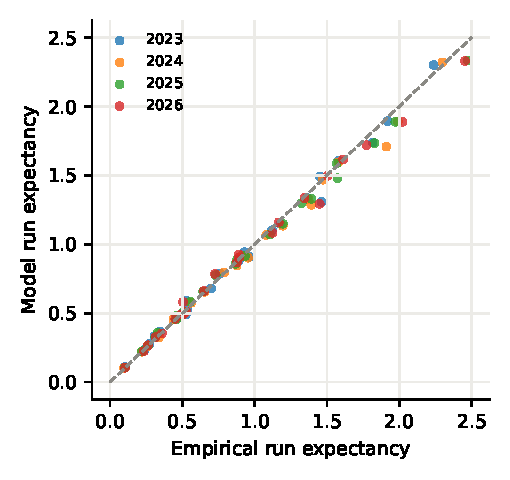
\includegraphics[width=0.48\textwidth]{figures/re24.pdf}\hfill
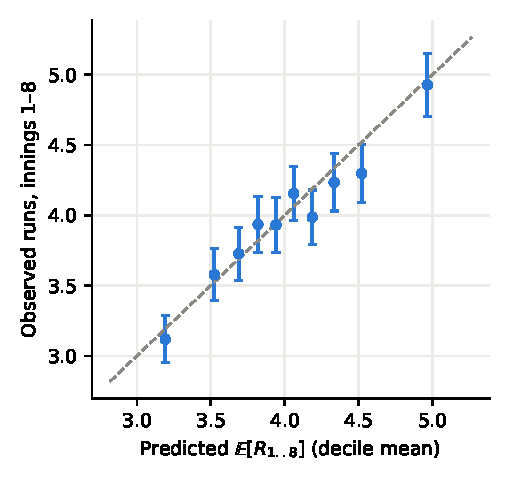
\includegraphics[width=0.48\textwidth]{figures/calibration.pdf}
\caption{Left: model versus empirical run expectancy for the 24 base-out states, 2023--2026 (E1).
Right: observed runs in innings 1--8 versus predicted expected runs, by decile of the prediction,
2025--2026 test seasons, with $\pm2$ standard errors (E3).}\label{fig:re24}\label{fig:calibration}
\end{figure}

\subsection{Plate-appearance model (E2)}

Tuning on 2024 selected prior-strength scales $\lambda_B=\EtwoBatterScale$,
$\lambda_P=\EtwoPitcherScale$ and half-life $H=\EtwoHalfLife$ days; the strength scales are
interior to the final grid, and $H=180$ days, evaluated in the first grid, was worse.
\Cref{tab:e2} reports the test seasons. Batter multipliers reduce log-loss relative to the league
model by about one hundredth of a nat per PA, and pitcher multipliers by a further 0.01; both
differences are large relative to their bootstrap intervals. Tuning the priors matters little
(about 0.001). The gradient-boosted model M3, using the same inputs, is better than M2 by 0.0008
nats in 2025 (interval excluding zero) and indistinguishable in 2026. Class-wise calibration of M2
is shown in \cref{fig:pacal}.

\begin{table}[t]\centering\small
\caption{Held-out log-loss (nats per PA) and difference from the full model with 95\% game-cluster bootstrap intervals. 2025: 186,562 PAs; 2026: 186,777 PAs.}\label{tab:e2}
\begin{tabular}{lcccc}\toprule
 & \multicolumn{2}{c}{2025} & \multicolumn{2}{c}{2026}\\
\cmidrule(lr){2-3}\cmidrule(lr){4-5}
Stage & Log-loss & $\Delta$ vs full & Log-loss & $\Delta$ vs full\\ \midrule
League rates & 1.7724 & $+$0.0278 [$+$0.0267, $+$0.0289] & 1.7735 & $+$0.0265 [$+$0.0255, $+$0.0276] \\
+ batter & 1.7547 & $+$0.0102 [$+$0.0095, $+$0.0109] & 1.7563 & $+$0.0093 [$+$0.0087, $+$0.0100] \\
+ pitcher (full model) & 1.7446 & --- & 1.7470 & --- \\
\bottomrule\end{tabular}\end{table}


\paragraph{Deviation from the pre-specified selection rule.} Our protocol selected the simplest
model not significantly worse than the best; strictly applied to 2025, it would select M3. We kept
M2 for the lineup analysis and report this as a deviation, for two reasons that we checked
rather than assumed. First, M2 provides the posterior distribution used for parameter uncertainty
(\cref{sec:uncertainty}), which M3 does not. Second, the choice does not change the decisions: on
\EtwocN{} random test team-games, the optimal order under M2 coincides with the M3 optimum in
\EtwocSame{} of the games, the M2 optimum loses on average \EtwocLoss{} runs per game when
evaluated under M3 (maximum \EtwocLossMax{}), the mean gains over the actual order are
\EtwocUpTwo{} (M2) and \EtwocUpThree{} (M3), and the correlation between the two models' values
over all 9! orders averages \EtwocCorr{}.

\paragraph{The original model.} On the window where its stored features exist (\EtwobWindow{},
\EtwobN{} PAs, which are out of sample for it), the predecessor system's 51-feature LightGBM has
log-loss \EtwobLegacyLL{} on the common seven-class taxonomy, against \EtwobMtwoLL{} for M2 and
\EtwobMzeroLL{} for the league model: M2 is better by \EtwobDiff{} nats per PA (95\% interval
\EtwobDiffLo{} to \EtwobDiffHi{}), despite the legacy features being recomputed daily rather than
every two weeks.

\begin{figure}[t]\centering
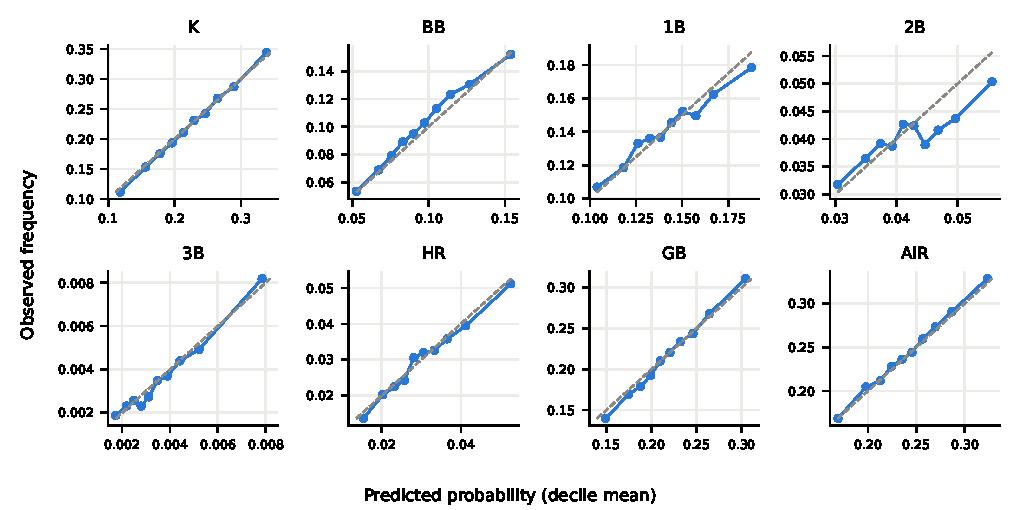
\includegraphics[width=\textwidth]{figures/pa_calibration.pdf}
\caption{Class-wise calibration of M2 on 2026 (deciles of the predicted probability).}\label{fig:pacal}
\end{figure}

\subsection{Run predictions at the game level (E3)}

Over \EthreeN{} test team-games, the mean prediction error (observed minus predicted runs in
innings 1--8) is \EthreeBias{} runs (95\% interval \EthreeBiasLo{} to \EthreeBiasHi{}), and the
calibration slope is \EthreeSlope{} (95\% interval \EthreeSlopeLo{} to \EthreeSlopeHi{}); neither
indicates miscalibration (\cref{fig:calibration}). The mean squared error is \EthreeMseModel{},
compared with \EthreeMseConst{} for the previous season's league mean and \EthreeMseTeam{} for
the team's mean over its previous 60 games. The correlation between predicted and observed runs
is only \EthreeCorr{}: almost all of the variance of a single game's runs is unpredictable before
the game. Randomized PIT values of the exact predicted run distributions on \EthreePitN{} random
team-games are close to uniform, and the central 80\% predictive interval covers
\EthreeCoverage{} of outcomes (\cref{fig:pit}); with integer-valued outcomes and inclusive interval
endpoints, coverage slightly above nominal is expected.

\begin{figure}[t]\centering
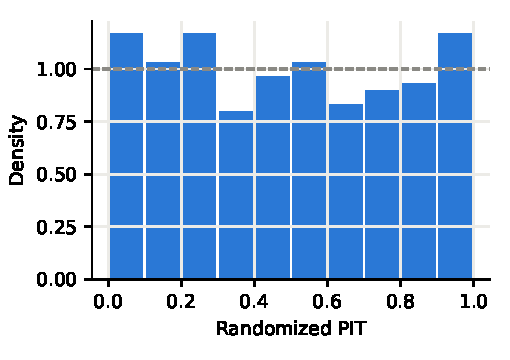
\includegraphics[width=0.48\textwidth]{figures/pit.pdf}
\caption{Randomized PIT histogram of observed runs in innings 1--8 (E3).}\label{fig:pit}
\end{figure}

\subsection{Search methods (E4a)}

\Cref{tab:e4a} compares the search methods with the exhaustive optimum. Exhaustive search takes
\EfouraExhaustiveSeconds{}~s per instance on one machine (all 362{,}880 orders). Local search from
ten random starts found the optimum in every instance tested, and simulated annealing and the
genetic algorithm with exact fitness came close, so for this problem size the choice among
competent search methods is unimportant once the objective is exact; exhaustive search is
preferred because it provides the certificate of \cref{cor:cert}. The heuristic guideline of
\citet{tango2007} recovers about half of the gap between the actual order and the optimum.

The genetic algorithm with Monte Carlo fitness, as in the predecessor system, performs worse
than the managers' own orders (mean gap \EfouraNoisyGap{} runs), and its reported value of the
chosen order exceeds the order's exact value by \EfouraCurse{} runs on average
(\EfouraNoisyN{} instances): the optimizer's curse is an order of magnitude larger than the
effect being optimized. With 4{,}000 simulated games, the standard error of one fitness evaluation
is about $3/\sqrt{4000}\approx0.05$ runs, larger than the differences among good orders.

\begin{table}[t]\centering\small
\caption{Search methods on 200 random 2026 regular-season team-games. Gap: exact $V(\pi^\star)-V(\hat\pi)$ in runs per game; Optimal: share of instances where the exact optimum was returned. $^\dagger$On 30 of them.}\label{tab:e4a}
\begin{tabular}{lrrrr}\toprule
Method & Mean gap & Max gap & Optimal & Evaluations\\ \midrule
Exhaustive search (exact) & 0.0000 & 0.0000 & 100\% & 362,880 \\
2-swap local search, 10 starts & 0.0000 & 0.0000 & 100\% & 1,933 \\
Simulated annealing & 0.0000 & 0.0021 & 94\% & 1,707 \\
Genetic algorithm, exact fitness & 0.0001 & 0.0034 & 82\% & 523 \\
2-swap local search from actual order & 0.0004 & 0.0091 & 68\% & 203 \\
\citeauthor{tango2007} guideline & 0.0092 & 0.0251 & 0\% & 0 \\
Sort by run value & 0.0092 & 0.0306 & 1\% & 0 \\
Sort by on-base probability & 0.0110 & 0.0341 & 0\% & 0 \\
Order actually used & 0.0186 & 0.0641 & 0\% & 0 \\
Original GA, Monte Carlo fitness$^\dagger$ & 0.0223 & 0.0526 & 0\% & 1,710 \\
\bottomrule\end{tabular}\end{table}


\subsection{How far are real orders from the optimum? (E4b)}

Across \EfourbN{} team-games of 2025--2026, the model-optimal order exceeds the order actually used
by \EfourbUpliftMean{} expected runs per game on average (median \EfourbUpliftMedian{}, 90th
percentile \EfourbUpliftQninety{}, maximum \EfourbUpliftMax{}), or \EfourbUpliftSeason{} runs per
162 games if the gap persisted every day (\cref{fig:uplift}). The best and the worst of all 9!
orders differ by only \EfourbSpread{} runs per game on average, and the optimum exceeds the average
of a uniformly random order by \EfourbOptVsRandom{}. Orders actually used rank, on median, above
\EfourbPctMedian{} of all possible orders, and \EfourbShareAboveNinety{} of them are above the 90th
percentile. In this model, therefore, managers' orders are close to optimal and the room for
improvement is a few runs per season, in line with the classical literature
\cite{freeze1974,tango2007}.

\begin{figure}[t]\centering
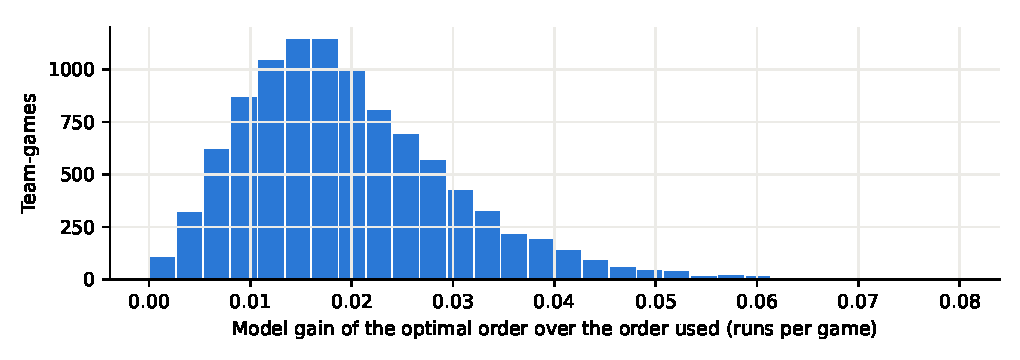
\includegraphics[width=\textwidth]{figures/uplift_hist.pdf}
\caption{Model gain of the optimal order over the order actually used, 2025--2026 (E4b).}\label{fig:uplift}
\end{figure}

\subsection{Parameter uncertainty}\label{sec:uncertainty}

In \EfourcN{} random 2026 team-games with \EfourcDraws{} posterior draws each (E4c), the point-
estimate optimal order is better than the actual order in \EfourcPBetter{} of draws on average,
but the 90\% posterior interval of the gain excludes zero in only \EfourcExcl{} of games, and its
mean width (\EfourcWidth{} runs) exceeds the typical gain. The exact optimal order changes in almost
every draw (it is unchanged in \EfourcSame{} of draws): many orders are nearly tied, and the data
cannot single out one of them. What the data do support is a statement about a set of good orders
(those that move the best hitters up), not about a unique best order.

\subsection{The 2026 World Series, Game 5 (E5)}

Milwaukee won 4--1 at Tropicana Field. Facing Drew Rasmussen and the Tampa Bay bullpen, the order
Milwaukee used has model value \RefActualAway{} expected runs over nine innings; the optimal order
\RefOptimalAway{} (gain \RefUpliftAway{}, 90\% interval \RefLoAway{} to \RefHiAway{}, optimal
better in \RefPBetterAway{} of \RefDraws{} posterior draws). The order used ranks above
\RefPctAway{} of all orders. For Tampa Bay, facing Jacob Misiorowski and the Milwaukee bullpen, the
values are \RefActualHome{} and \RefOptimalHome{} (gain \RefUpliftHome{}, interval \RefLoHome{} to
\RefHiHome{}, better in \RefPBetterHome{} of draws; rank \RefPctHome{}). The observed scores
(\RefObservedAway{} and \RefObservedHome{} runs) are single draws from predictive distributions
with a standard deviation of about three runs and carry essentially no information about the
merit of either order (\cref{rem:identification}). \Cref{tab:ref} lists the orders.

\begin{table}[t]\centering\small
\caption{2026 World Series Game 5: starting orders used and model-optimal orders (information before 2026-10-28).}\label{tab:ref}
\begin{tabular}{rllll}\toprule
 & \multicolumn{2}{c}{Milwaukee Brewers} & \multicolumn{2}{c}{Tampa Bay Rays}\\
\cmidrule(lr){2-3}\cmidrule(lr){4-5}
Slot & Used & Optimal & Used & Optimal\\ \midrule
1 & Jackson Chourio & Brice Turang & Yandy Díaz & Liam Hicks \\
2 & Jake Bauers & Jake Bauers & Jonathan Aranda & Jonathan Aranda \\
3 & Christian Yelich & William Contreras & Junior Caminero & Junior Caminero \\
4 & William Contreras & Jackson Chourio & Liam Hicks & Yandy Díaz \\
5 & Brice Turang & Cooper Pratt & Jonny DeLuca & Chandler Simpson \\
6 & Sal Frelick & Christian Yelich & Chandler Simpson & Ryan Vilade \\
7 & Cooper Pratt & Garrett Mitchell & Ben Williamson & Jonny DeLuca \\
8 & Garrett Mitchell & Sal Frelick & Ryan Vilade & Ben Williamson \\
9 & David Hamilton & David Hamilton & Taylor Walls & Taylor Walls \\
\bottomrule\end{tabular}\end{table}



%======================================================================
\section{Sensitivity, limitations and threats to validity}\label{sec:sensitivity}
%======================================================================

\paragraph{Parameter uncertainty.} The Gamma posteriors describe sampling uncertainty in player
multipliers under a working Poisson likelihood; they do not include uncertainty in the kernel,
the starter-workload curve, or model misspecification, and draws are independent across classes
and players. The weighted working likelihood, on the other hand, overstates the sampling
variance of decayed counts, and kernel uncertainty is shared by all orders and partly cancels in
differences. The reported intervals are therefore likely, but not guaranteed, to understate total
uncertainty.

\paragraph{Misspecification.} \Cref{as:kernel} ignores runner speed and individual double-play
tendencies beyond ground-ball rate; fast runners make the leadoff slot more valuable than the
model suggests. \Cref{as:regime} places pitching changes between innings, whereas real changes
often happen mid-inning and respond to the score (and, through the times-through-the-order effect,
to the lineup). Platoon effects are league-level. In-game substitutions are ignored, which matters
most for slots 7--9 in the late innings.

\paragraph{Objective.} Maximizing expected runs is not the same as maximizing win probability;
in close late-game situations a manager may value the variance of runs differently. We do not
model this.

\paragraph{Data.} Statcast occasionally revises recent games; decisive-pitch states may contain
scorer errors (removed when they violate bookkeeping: \DataErrMin--\DataErrMax{} transitions per season outside
the censored ones, \cref{tab:data}). Lineups for the
backtests are inferred (\EzeroMatch{} of \EzeroN{} matched the official boxscore in the E0 audit),
with no guarantee for every game.

\paragraph{Counterfactuals.} As stated in \cref{rem:identification}, none of the comparisons
between orders is an observed effect.

%======================================================================
\section{Conclusions}
%======================================================================

Under explicit Markov assumptions, the expected runs of a batting order can be computed exactly and
cheaply, which turns batting-order optimization from a noisy search into an exhaustive one with a
certificate. With an empirical-Bayes plate-appearance model that uses only pregame information,
the model's run predictions are calibrated on two held-out seasons, and the simple model predicts
plate appearances about as well as a gradient-boosted classifier given the same inputs.

The substantive conclusion is modest and, we think, robust: in this model the batting orders that
MLB teams actually used in 2025--2026 were close to optimal (median rank above \EfourbPctMedian{}
of all orders), and reordering would add about \EfourbUpliftMean{} expected runs per game, roughly
\EfourbUpliftSeason{} runs over a season. On average, the best and worst possible orders of the
same nine hitters differ by less than a tenth of a run per game (\EfourbSpread{}). For the 2026 World Series Game 5 the
estimated gains were \RefUpliftAway{} (Milwaukee) and \RefUpliftHome{} (Tampa Bay) runs, with
parameter uncertainty of the same size, and the identity of the single best order is not
statistically determined. Both orders were near-optimal: for Tampa Bay the model's preferred order is better
with high posterior probability (\RefPBetterHome{} of draws), but by only \RefUpliftHome{} runs per
game, and for Milwaukee the gain's interval includes zero. The actual result of the game cannot speak
to either question.

What remains uncertain is everything outside the model: base-running speed, mid-inning pitching
changes, individual platoon effects and in-game substitutions. Each of these could change the
ranking of nearly tied orders; we expect none of them to change the order of magnitude of the
effect. The method itself is the paper's practical contribution: a reproducible, leakage-free
pipeline and an exact optimizer, with an interactive public interface that runs the same
computation in the browser.


\bibliographystyle{plainnat}
\bibliography{references}

\appendix
\section{Reproducibility}\label{app:repro}

\begin{verbatim}
pip install -e ".[ingest,compare,figures,dev]"
batting-order ingest 2021 2022 2023 2024 2025 2026   # Baseball Savant, resumable
batting-order build  2021 2022 2023 2024 2025 2026
batting-order experiments                             # writes outputs/*.json
python scripts/make_paper_assets.py                   # figures + generated/*.tex
cd research && latexmk -pdf paper.tex
\end{verbatim}
Raw files are verified against \texttt{data/raw/statcast/season=*/MANIFEST.json}.
The numerical claims of \cref{sec:model} are covered by tests: closed-form checks (an out/home-run
model where runs per inning are negative binomial with mean $3(1-q)/q$), agreement with an
independently written Monte Carlo simulator, agreement of the exact distribution's mean with
\eqref{eq:value}, the truncation bound of \cref{prop:trunc}, and parity of the browser
implementation with the reference implementation to $10^{-10}$.

\section{Run expectancy, 2026}\label{app:re24}
Model run expectancy (empirical in parentheses) by bases occupied and outs; 2026 kernel with the league outcome mix. Bases: 1 = first, 2 = second, 3 = third.

\begin{center}\small\begin{tabular}{lccc}\toprule
Bases & 0 outs & 1 out & 2 outs\\ \midrule
--- & 0.491 (0.493) & 0.267 (0.263) & 0.104 (0.104) \\
1-- & 0.868 (0.877) & 0.513 (0.526) & 0.222 (0.232) \\
-2- & 1.082 (1.122) & 0.661 (0.650) & 0.327 (0.314) \\
12- & 1.496 (1.503) & 0.924 (0.891) & 0.459 (0.451) \\
--3 & 1.293 (1.450) & 0.904 (0.893) & 0.354 (0.359) \\
1-3 & 1.719 (1.773) & 1.159 (1.167) & 0.489 (0.504) \\
-23 & 1.888 (2.022) & 1.335 (1.344) & 0.581 (0.504) \\
123 & 2.330 (2.454) & 1.614 (1.611) & 0.785 (0.726) \\
\bottomrule\end{tabular}\end{center}


\end{document}
